In this section, we describe our empirical evaluation of the EAGER
prototype and evaluate its overhead and scaling characteristics.
To do so, we populate the EAGER database (Metadata Manager) with a 
set of APIs, and examine
the overheads associated with governing a set of sample applications 
for varying degrees of policy specifications and dependencies.

Note that all the figures included in this section present the average values calculated
over three sample runs. The error bars cover an interval of two standard deviations centered
at the calculated sample average. Also, our experiments have shown that the absolute
overhead introduced by EAGER is very small compared to the overall time taken by
AppScale to deploy an application (100's of milliseconds as opposed
to 10's of seconds). Therefore, for clarity and ease of comparison, all the figures presented 
in this section only show the absolute overhead of EAGER.

Figure~\ref{fig:overhead_by_apis} shows that EAGER overhead grows linearly
with the number of APIs exported by a deployed application.  This scaling occurs
because the current prototype implementation iterates through the APIs in the
application sequentially and records the API metadata in the Metadata Manager.
Then EAGER publishes each API to the ADP and API Gateway. This sequencing of
individual EAGER events, each of which generates a separate web service call,
represents an optimization opportunity via parallelization in future implementations.

\begin{figure}
\centering
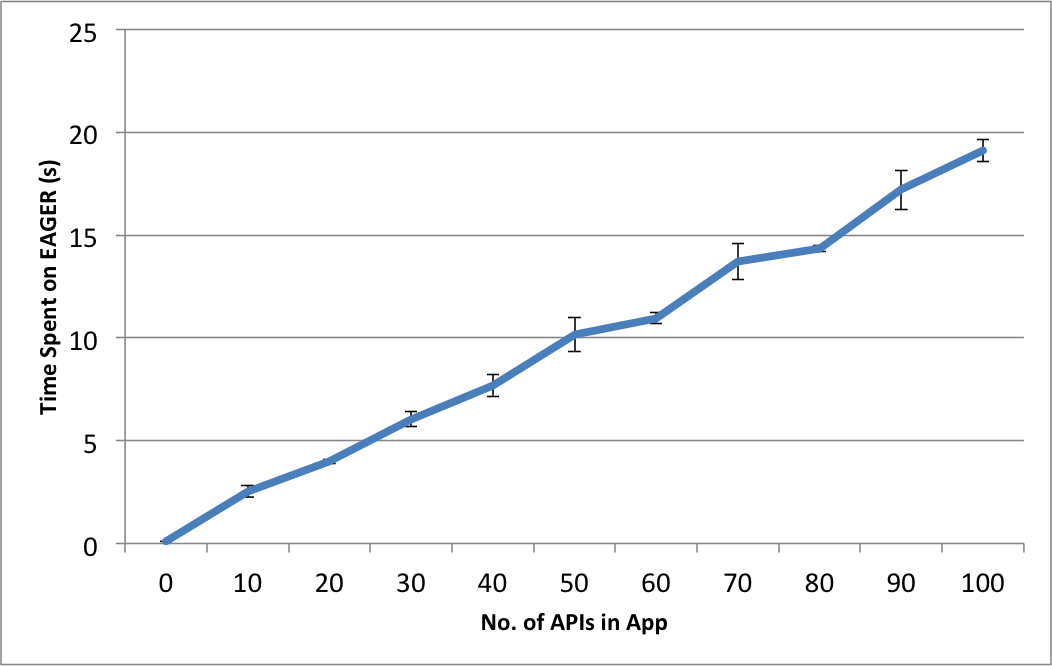
\includegraphics[scale=0.47]{overhead_by_apis}
%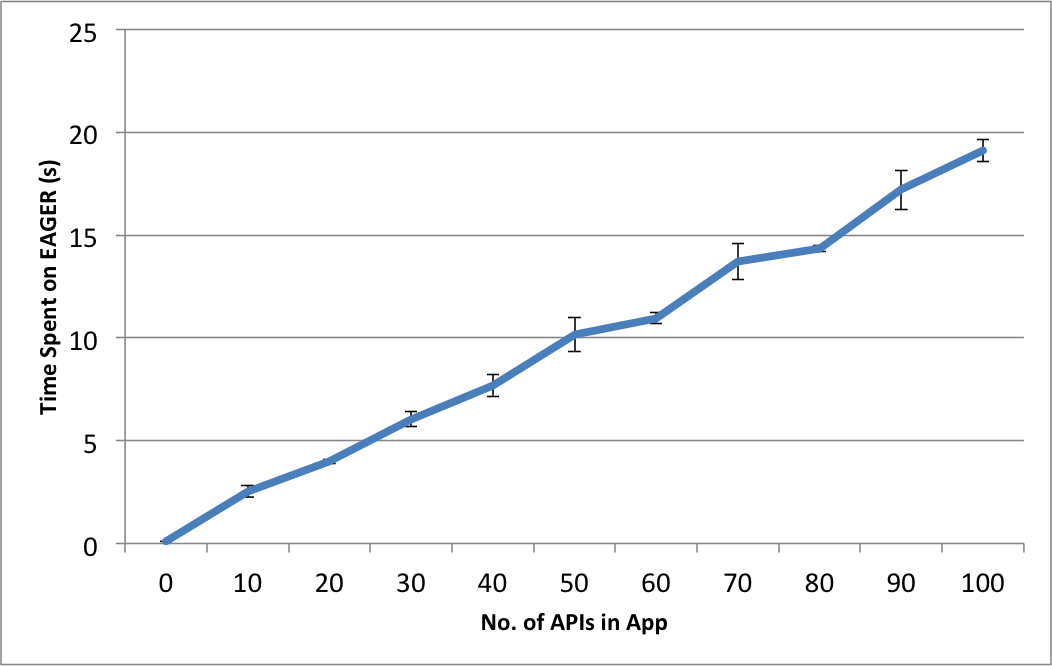
\includegraphics[width=3in]{overhead_by_apis}
%\vspace{-0.01in}
\caption{Average EAGER overhead vs. number of APIs exported by the
application.}
\label{fig:overhead_by_apis}
\vspace{-0.2in}
\end{figure}

At present we expect most applications deployed in cloud to have a small to 
moderate number of APIs ($10$ or fewer).  With this API density EAGER's current 
scaling is adequate.  Even in the
unlikely case that a single application exports as many as $100$ APIs,
the average total time for EAGER is under $20$ seconds.

Next, we analyze EAGER overhead as the number of dependencies declared in
an application grows. For this experiment, we first populate the EAGER
Metadata Manager with metadata for $100$ randomly 
generated APIs.
Then we
deploy an application on EAGER which exports a single API and declares
artificial dependencies on the set of fictitious 
APIs that are already stored in the Metadata Manager. We
vary the number of declared dependencies and observe the EAGER overhead.

\begin{figure}
\centering
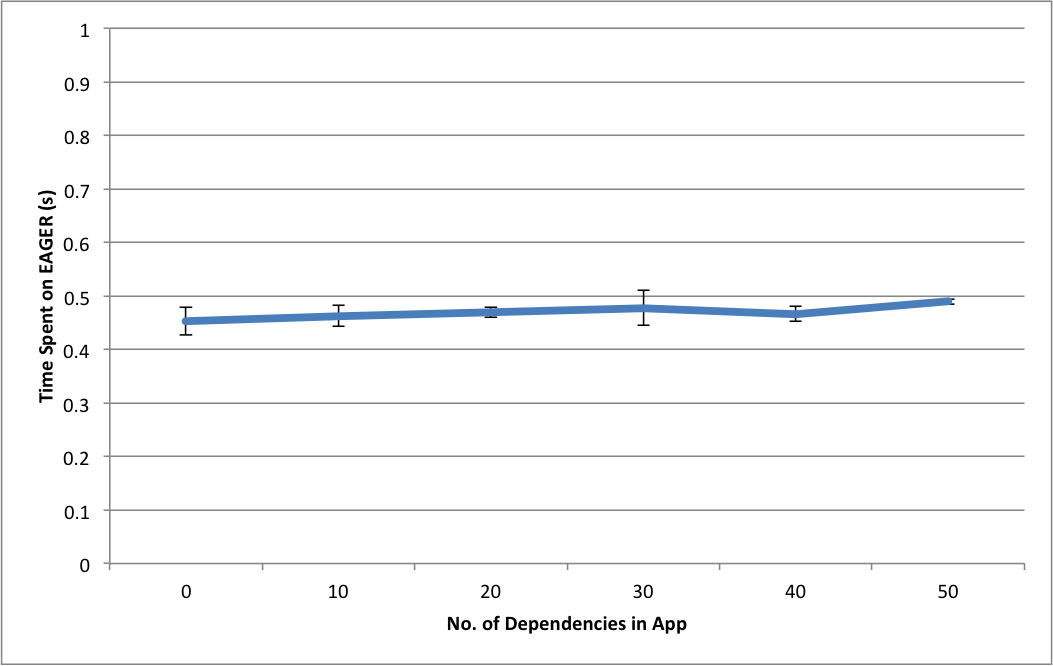
\includegraphics[scale=0.47]{overhead_by_deps}
%\vspace{-0.01in}
\caption{Average EAGER Overhead vs. number of dependencies declared in the
application.}
\label{fig:overhead_by_deps}
\vspace{-0.2in}
\end{figure}

Figure~\ref{fig:overhead_by_deps} shows the results of these experiments. 
EAGER overhead does not appear to be significantly
influenced by the number of dependencies declared in an application. 
In this case, the EAGER implementation processes
all dependency-related information via batch operations. 
As a result, the number of web service calls and database queries that originate 
due to varying number of dependencies is fairly constant. 

So far we have conducted all our experiments without any active governance 
policies in the system. In this section, we report how EAGER overhead
is impacted by the number of policies.

The overhead of policy validation is largely dependent on the actual policy
content. Since users may include any Python code 
(as long as it falls in the accepted subset) in a policy file, evaluating a
given policy can take an arbitrary amount of time.  Therefore, in this
experiment, our goal is to evaluate the overhead incurred by simply having
many policy files to execute. We keep the content of the policies small and
trivial. We create a policy file that runs following assertions:
\begin{enumerate} 
\item Application name must start with an upper case letter
\item Application must be owned by a specific user 
\item All API names must start with upper case letters 
\end{enumerate} We create many copies of this
initial policy file to vary the number of policies deployed. Then we evaluate
the overhead of policy validation on two of our sample applications
(guestbook-py and simple-jaxrs-app). 

\begin{figure}
\centering
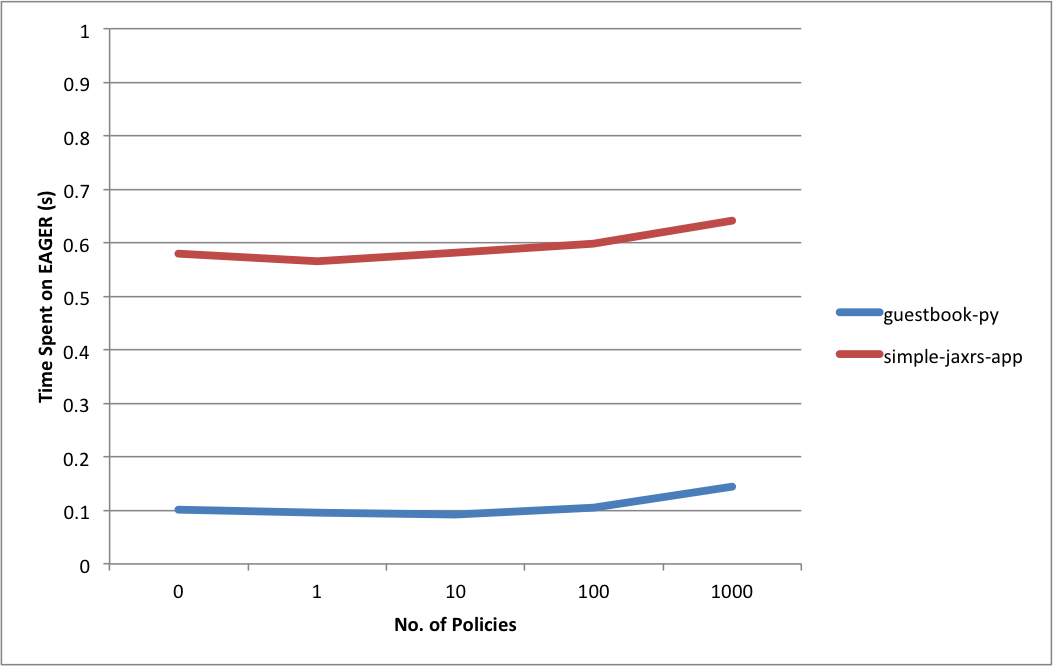
\includegraphics[scale=0.47]{overhead_by_policies}
%\vspace{-0.01in}
\caption{Average EAGER overhead vs. number of policies.Note that some of the error bars for 
guestbook-py are smaller than the graph features at this scale and are thus obscured.}
\label{fig:overhead_by_policies}
\vspace{-0.2in}
\end{figure}

Figure~\ref{fig:overhead_by_policies} shows how the number of active policies
impact EAGER overhead. Interestingly, even large numbers of policies 
do not impact EAGER overhead significantly. It is only when the active
policy count approaches $1000$ that we can see a small increase in the
overhead. Even then, the increase in deployment time is under $0.1$ seconds. 

This result is due to the fact that EAGER loads policy content into memory at system
startup (or when a new policy is deployed), and executes them from memory each
time an application is deployed. Since policy files are typically small (at
most a few kilobytes), this is a viable option. The overhead of validating the
simple-jaxrs-app is higher than that of the guestbook-py because,
simple-jaxrs-app exports two web APIs whereas guestbook-py exports none. 

Next, we evaluate how EAGER scales when a large number of APIs are deployed 
in the cloud. In this experiment, we populate the EAGER
Metadata Manager with a varying number of random APIs. We then attempt to deploy various sample 
applications. We also create random dependencies among the APIs recorded in the 
Metadata Manager to make the experimental setting more realistic.

\begin{figure}
\centering
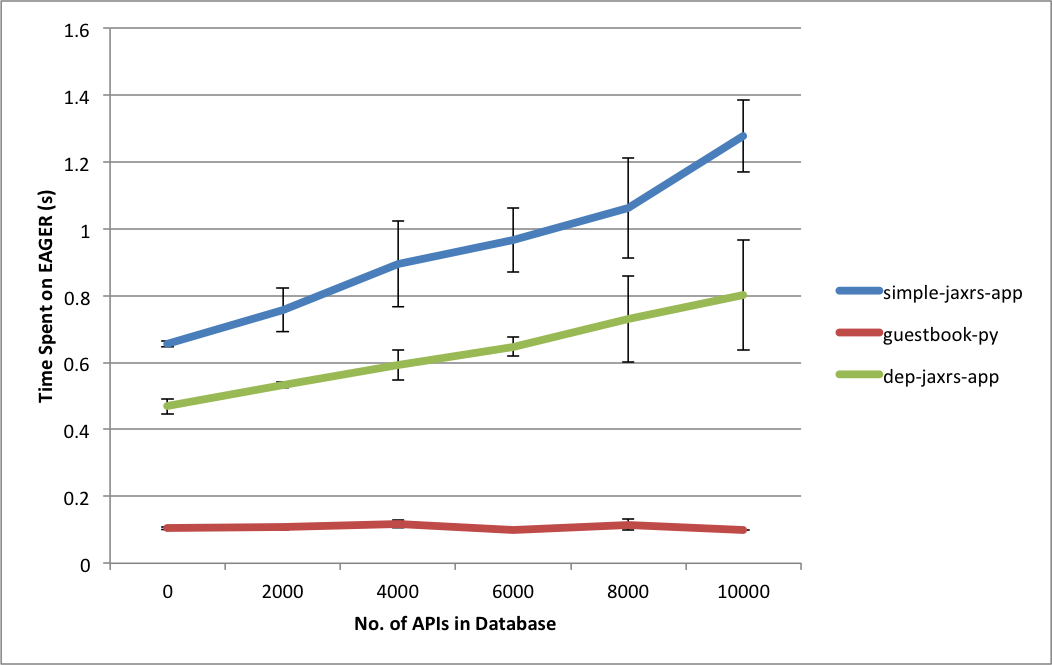
\includegraphics[scale=0.47]{scalability}
%\vspace{-0.01in}
\caption{Average EAGER overhead vs. number of APIs in Metadata Manager. Note that some of the error bars for
guestbook-py are smaller than the graph features at this scale and are thus obscured.}
\label{fig:scalability}
\vspace{-0.2in}
\end{figure}

Figure~\ref{fig:scalability} shows that the deployment overhead of the 
guestbook-py application is not impacted by the growth of metadata
in the cloud. Recall that guestbook-py does not export any APIs nor does it 
declare any dependencies. Therefore the deployment process of
the guestbook-py application has minimal interactions with the 
Metadata Manager. Based on this result we conclude that applications that
do not export web APIs are not significantly affected by the accumulation 
of API metadata in EAGER.

Both simple-jaxrs-app and dep-jaxrs-app are
affected by the volume of data stored in Metadata Manager. Since these applications 
export web APIs that must be recorded and validated by the Metadata Manager, 
the growth of metadata has an increasingly higher impact on them. 
The degradation 
of performance as a function of the number of APIs in the Metadata Manager
database is due to the slowing of query performance of the RDBMS engine (MySQL) 
as the database size grows. Note that the simple-jaxrs-app
is affected more by this performance drop, because it exports two APIs compared to the single API exported 
by dep-jaxrs-app. However, the growth
in overhead is linear to the number of APIs deployed in the cloud. Also,
even after deploying $10000$ APIs, the overhead on simple-jaxrs-app is only been increased by 
about $0.5$ seconds.

In summary, the current EAGER prototype scales well to $1000$'s of APIs.
If further scalability is required, we can employ
parallelization and data storage-level optimizations.
EAGER adds a very small overhead to the application deployment
process, and 
this overhead increases linearly with the number of APIs exported by the applications
and the number of APIs deployed in the cloud. 
Interestingly, the number of deployed policies and declared dependencies
have little impact on the EAGER governance overhead. Based on this analysis we
can conclude that enforced deployment-time API governance can be implemented in modern PaaS
clouds with negligible overhead and very high scalability. Further, deployment-time API governance
can be made an intrinsic component of the PaaS cloud itself thus alleviating the need
for poorly integrated third party API management solutions.